\documentclass[9pt]{beamer}

\usepackage[francais]{babel}
\usepackage[T1]{fontenc}
\usepackage[utf8]{inputenc}     % utf8
\usepackage{verbatim}           %pour \verbatiminput{fich}
\usepackage{wasysym}
\usepackage{blindtext}
\usepackage{eurosym} 
\usepackage{epigraph}

\usetheme{Madrid}    % titre en haut
\usetheme{Frankfurt}

\graphicspath{{figures/}}
\setbeamertemplate{caption}[numbered] % pour numéroter tables et figures !
%si \verb   : \begin{frame}[fragile]
%si verbatim  : \begin{frame}[containsverbatim]

\title[Blob Wars]{HLIN405 - Projets de Programmation de L2\\\vspace{5px}-----------\vspace{4px}\\\huge \textbf{Blob Wars}\vspace{3px}\\}

\author[Allouch, Roux, Villaroya]{ 
Allouch Yanis
\and 
Roux Jérémie
\and 
Villaroya Kévin
 }
 
\institute[UM - FdS]{2018 - 2019}

\date[21 mai 2019]{Université de Montpellier - Faculté des Sciences}


%%%%%%%%%%%%%%%%%%%%%%%%%%%%%%%%%%%%%%%%%%%%%%%%%%%
%%%%%%%%%%%%%%%%%%%%%%%%%%%%%%%%%%%%%%%%%%%%%%%%%%%
%%%%%%%%%%%%%%%%%%%%%%%%%%%%%%%%%%%%%%%%%%%%%%%%%%%


\begin{document}

\makeatletter
    \newenvironment{withoutheadline}{
        \setbeamertemplate{headline}[default]
        \def\beamer@entrycode{\vspace*{-\headheight}}
    }{}
\makeatother

\begin{withoutheadline}

    % Premier transparent de titre
    \begin{frame}
        \titlepage
    
        \begin{minipage}[c]{.1\linewidth}
            \begin{center}
                
\includegraphics[width=2.5cm]{./figures/facSciences.png}
            \end{center}
       \end{minipage} 
       \hfill
       \begin{minipage}[c]{.46\linewidth}
            \begin{center}
                
\includegraphics[width=3cm]{./figures/icone.png}
            \end{center}
        \end{minipage}
        \begin{minipage}[c]{.26\linewidth}
            \begin{center}
                
\includegraphics[width=3.2cm]{./figures/umontpellier.png}
            \end{center}
        \end{minipage}
    \end{frame}
    
\end{withoutheadline}

\begin{withoutheadline}
      
    % 2eme transparent TDM générale    
    \begin{frame}
        \frametitle{Table des matières}
        {\small \tableofcontents[]}
    \end{frame}

\end{withoutheadline}

\section{Introduction}

\subsection{Règles du jeu}

\begin{frame}[fragile]
\frametitle{\insertsectionhead : \insertsubsectionhead}

\begin{block}{Blob Wars, un jeu de plateau de type Othello}
\textbf{Condition de victoire :} Avoir le plus de pions à la fin de la partie\\
\textbf{Mécanique principale :} Se déplacer ou se cloner sur une case adjacente à un pion ennemi pour le convertir\\
\textbf{Fin de la partie :} Plateau rempli ou $n - 1$ joueurs ne peuvent plus bouger (soit $n$ le nombre de joueurs au total)
\end{block}

\begin{figure}[h]
\begin{center}
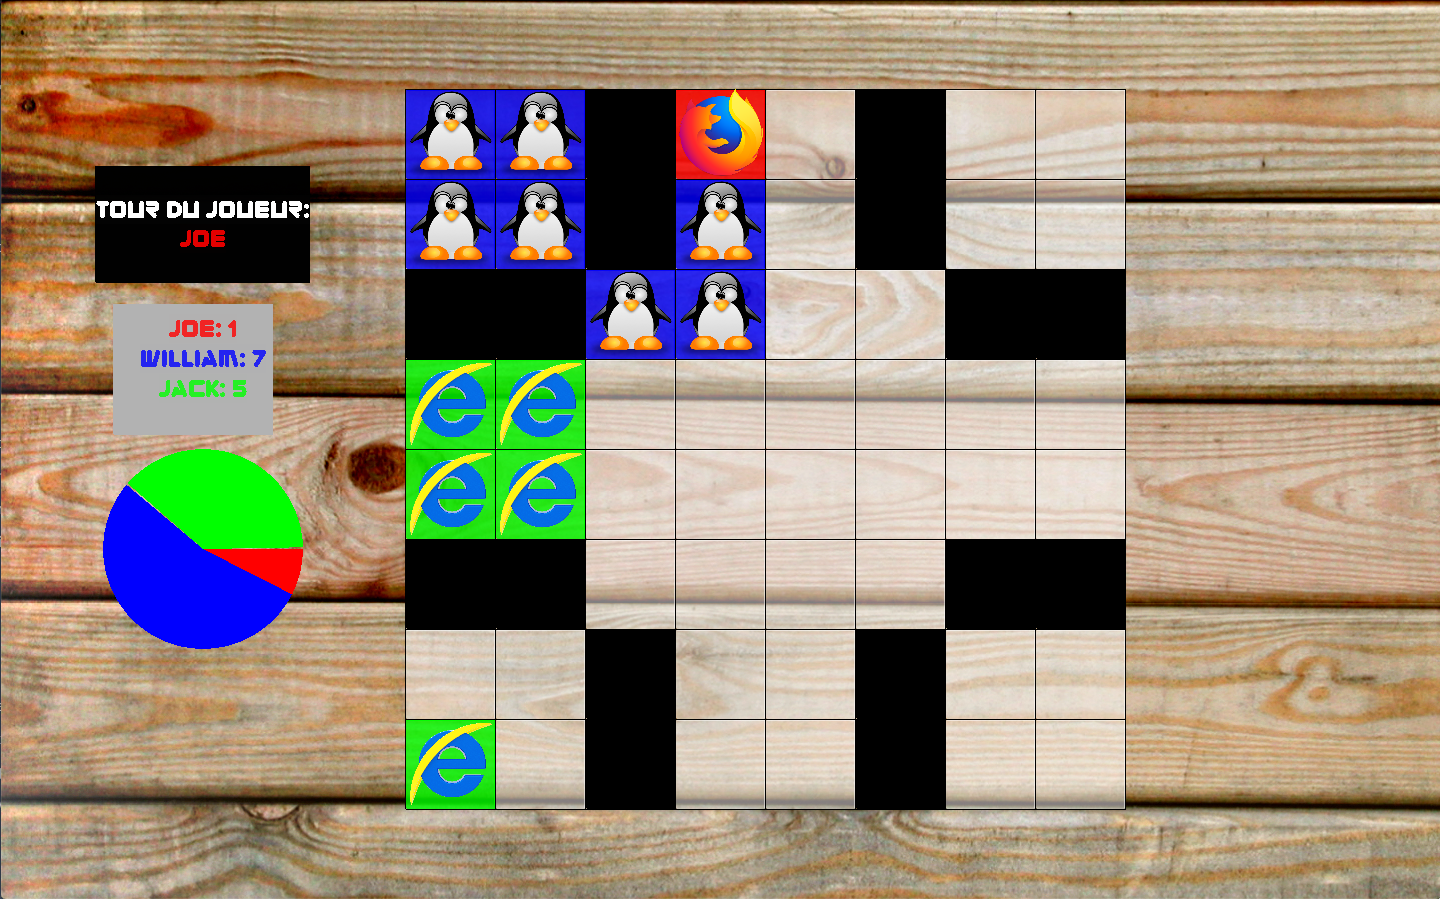
\includegraphics[width=0.55\textwidth]{captures/capturePartie.png}
\vspace{-5px}
\caption{Capture d'écran d'une partie avec notre application Blob Wars}
\end{center}
\end{figure}

\end{frame}

\subsection{Mécaniques de jeu}

\begin{frame}[fragile]
\frametitle{\insertsectionhead : \insertsubsectionhead}

\begin{columns}

\begin{column}{4cm}
\begin{center}
Analysons les 4 types de coups possibles du pingouin situé au centre de l'écran.
\vspace{10px}
\begin{block}{Mouvements possibles}
\textbf{1 :} Simple déplacement\\
\textbf{2 :} Déplacement et attaque\\
\textbf{3 :} Simple clonage\\
\textbf{4 :} Clonage et attaque\\
\end{block}
\begin{block}{Zones}
\textbf{Grise claire :} Déplacement\\
\textbf{Grise foncée :} Clonage\\
\end{block}
\end{center}
\end{column}

\begin{column}{7cm}
\begin{figure}[h]
        \begin{center}
            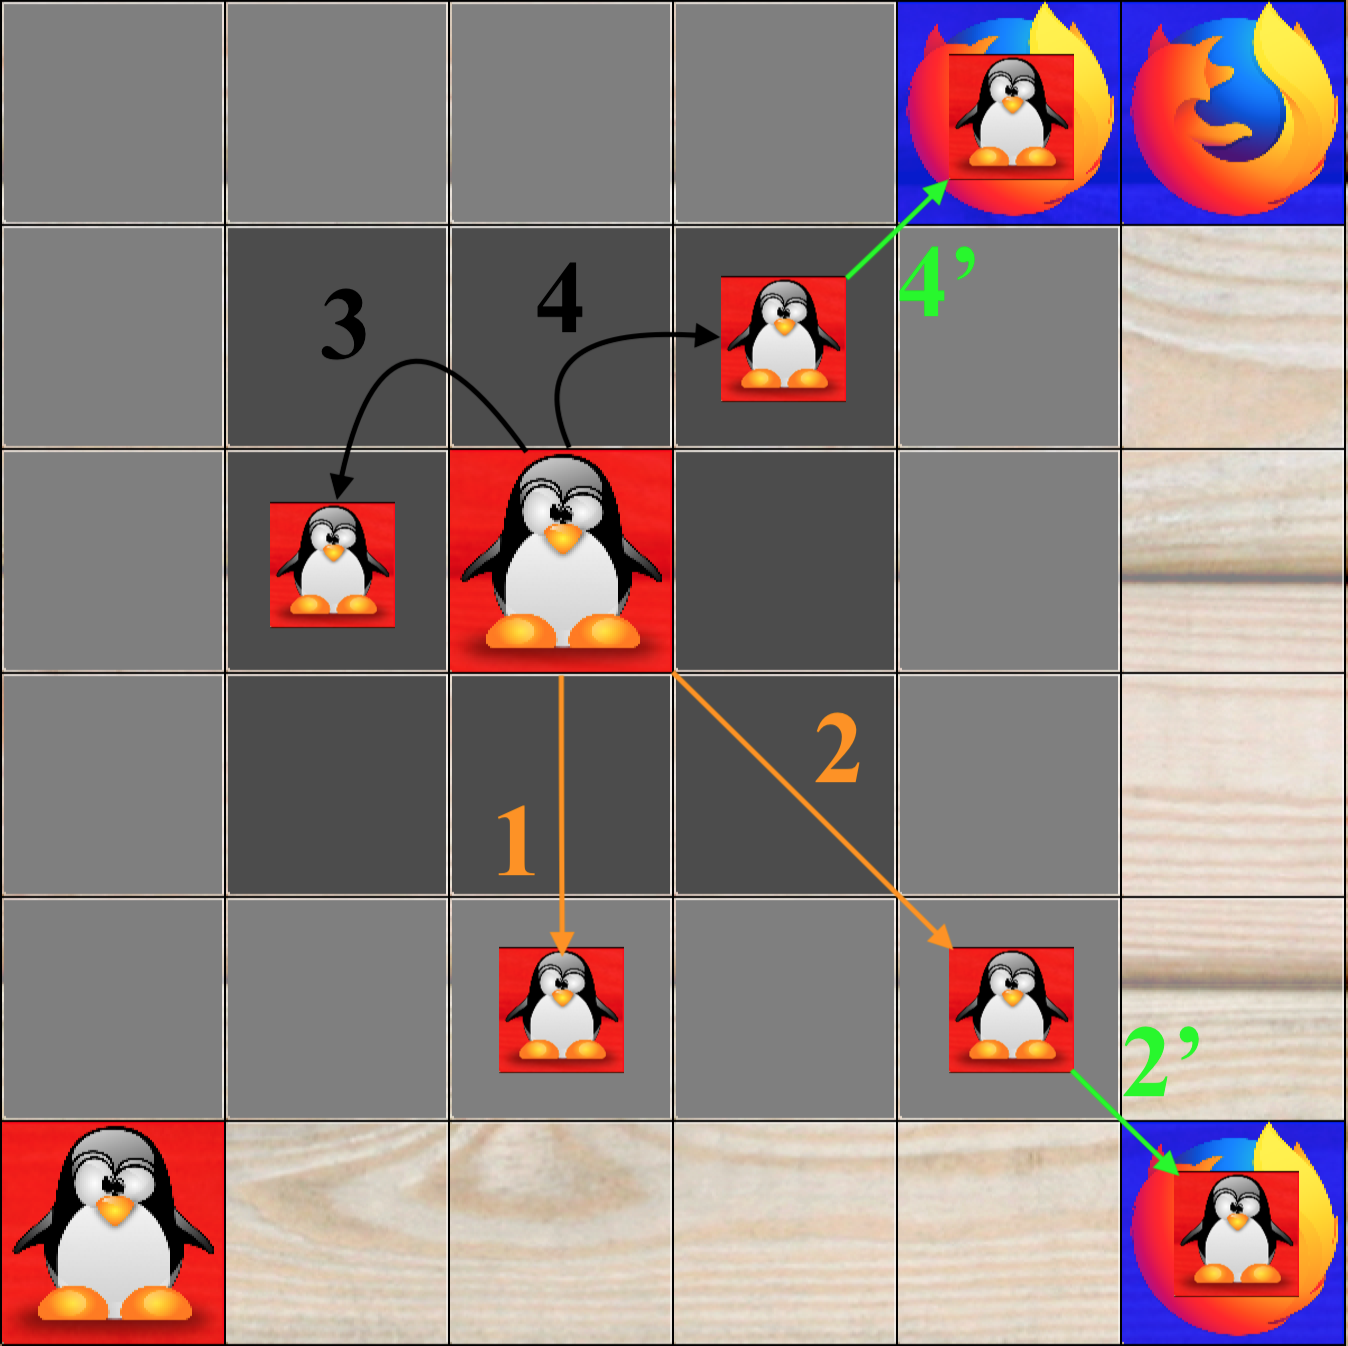
\includegraphics[width=0.9\textwidth]{figures/Situations.png}
            \caption{4 types de coups possibles}
        \end{center}
    \end{figure}
\end{column}

\end{columns}

\end{frame}

\section{Démonstration}

\begin{frame}
\frametitle{\insertsectionhead}

Voici une démonstration de l'application Blob Wars (développée en Java) que nous avons conçue.
\begin{figure}[h]
    \begin{center}
        
\includegraphics[width=0.35\textwidth]{figures/icone.png}
        \caption{Logo de notre application Blob Wars}
    \end{center}
\end{figure}
Dans notre version du Blob Wars, les "blobs" sont des logos de moteurs de recherche, de systèmes d'exploitations ou de marques.
\end{frame}

\section{Développement}

\subsection{Structure globale}

\begin{frame}[fragile]
\frametitle{\insertsectionhead : \insertsubsectionhead}
\begin{block}{Structure du programme}
La \textbf{fenêtre de jeu} (interface graphique) dialogue avec le \textbf{moteur du jeu} et \textbf{le jeu en lui-même}.
\end{block}
\begin{figure}[h]
    \begin{center}
        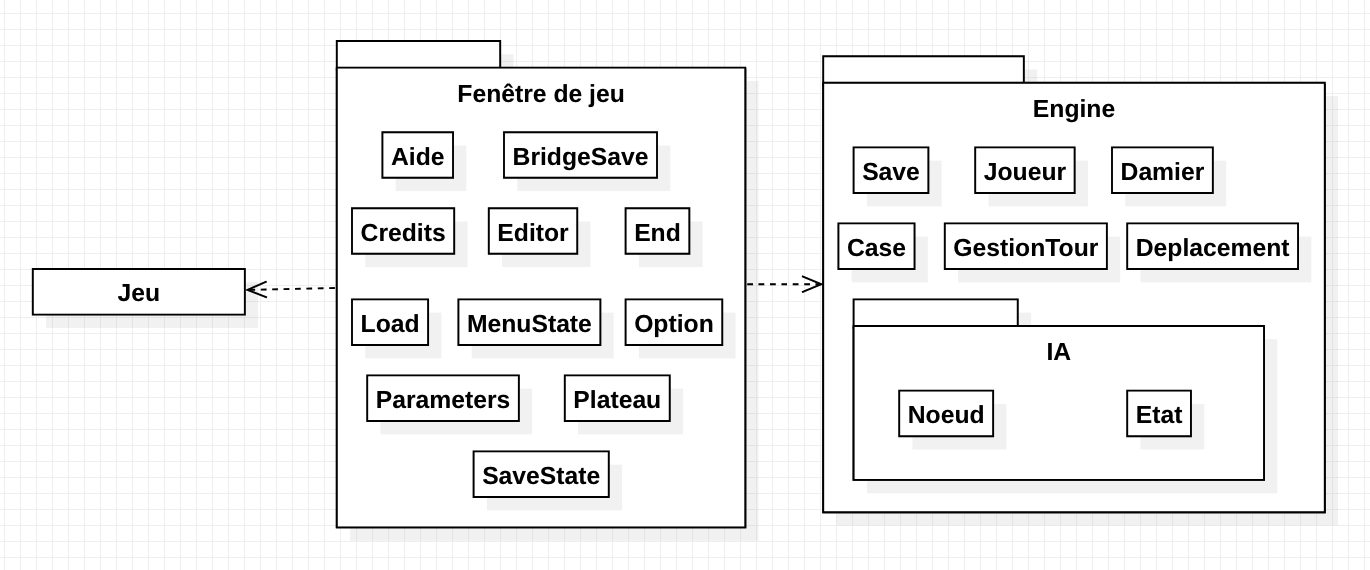
\includegraphics[width=1\textwidth]{figures/UML/diagramme_simp.png}
        \caption{Diagramme de classes simplifié global}
    \end{center}
\end{figure}
\end{frame}

\subsection{Fichiers de configuration}

\begin{frame}[fragile]
\frametitle{\insertsectionhead : \insertsubsectionhead}
L'utilisateur peut générer ou charger des fichiers de configuration afin de sauvegarder ou charger des parties.
\begin{figure}[h]
    \begin{center}
        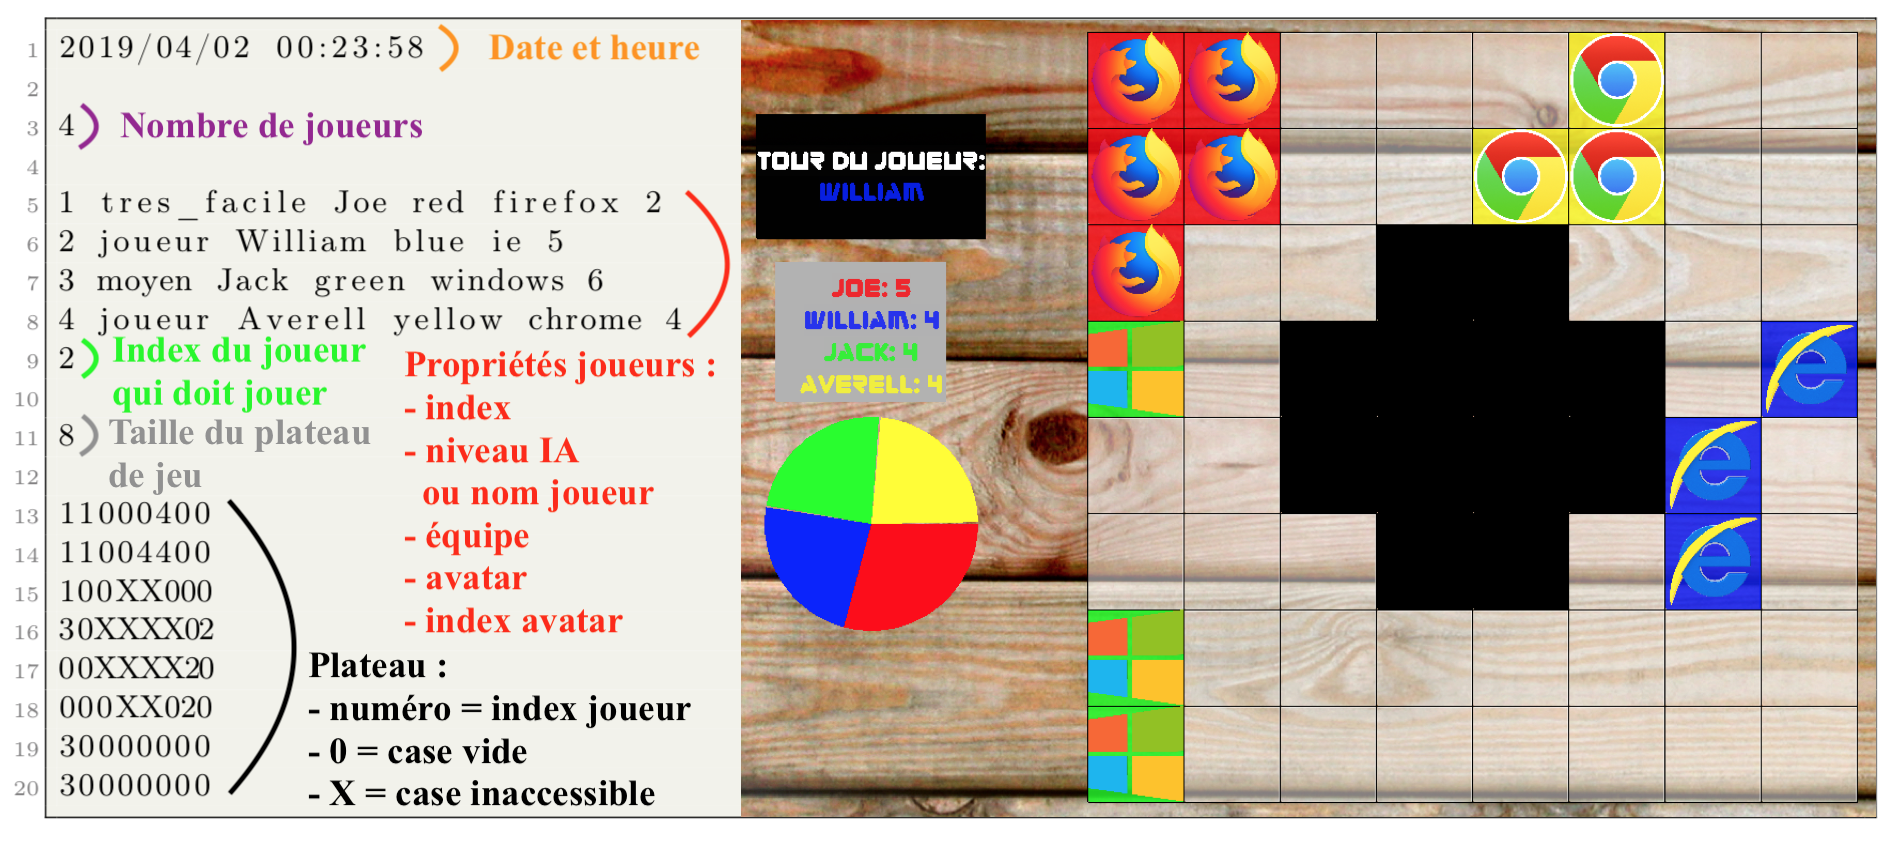
\includegraphics[width=1\textwidth]{figures/fichierconfig.png}
        \caption{Exemple d’un fichier de configuration et de la partie correspondante}
    \end{center}
\end{figure}
\end{frame}

\subsection{Musique et bruitages}

\begin{frame}[fragile]
\frametitle{\insertsectionhead : \insertsubsectionhead}
\begin{block}{Garage Band}
Il s'agit d'un logiciel de MAO (Musique Assistée par Ordinateur) avec lequel nous avons composé la musique et fabriqué les bruitages du jeu.
\end{block}
\begin{figure}[h]
    \begin{center}
        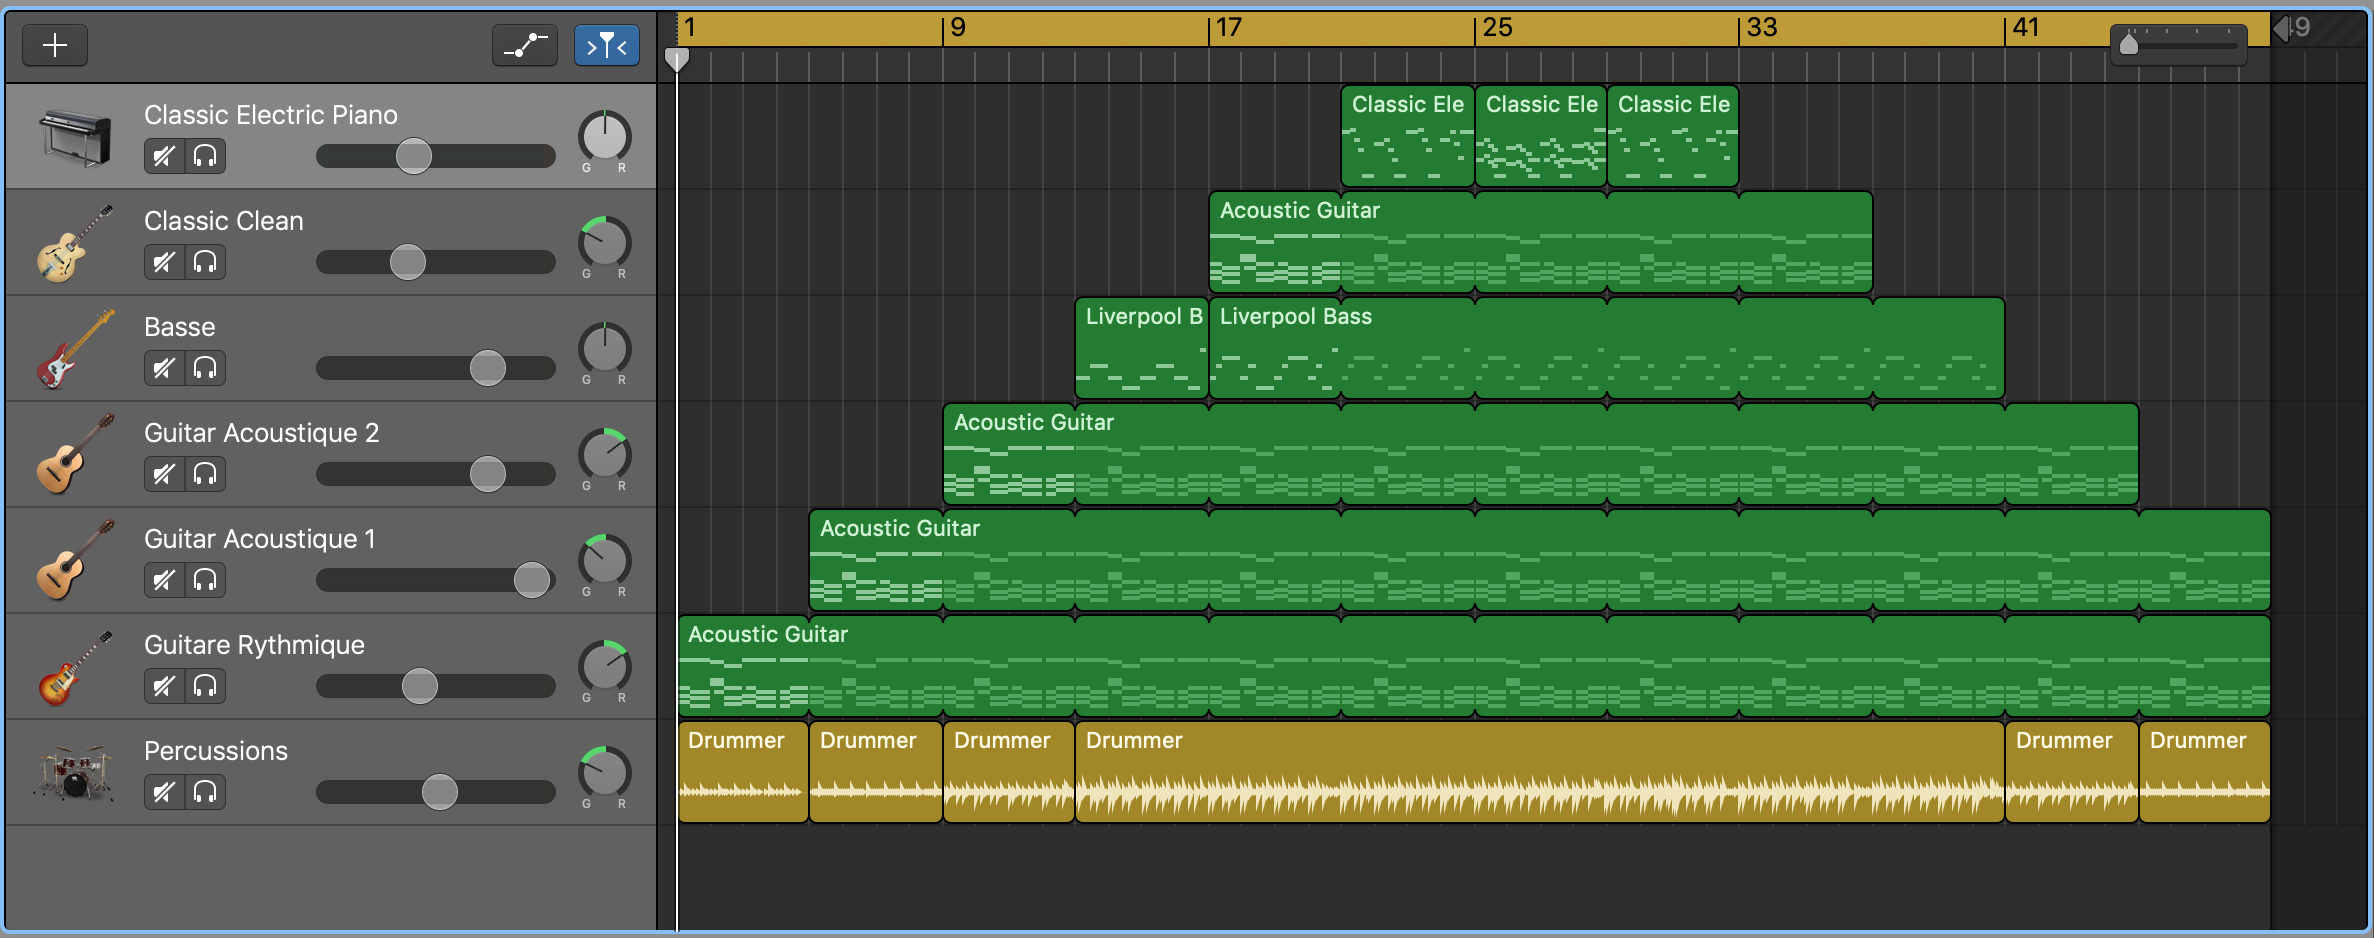
\includegraphics[width=1\textwidth]{figures/mao.png}
        \caption{Aperçu dans Garage Band de la bande originale du jeu Blob Wars}
    \end{center}
\end{figure}
\end{frame}

\section{Intelligence artificielle}

\subsection{Fonction d'évaluation}

\begin{frame}[fragile]
\frametitle{\insertsectionhead : \insertsubsectionhead}

\begin{columns}

\begin{column}{4cm}
\begin{center}
\begin{block}{Eval()}
La fonction attribue une valeur entière à un état de jeu pour un joueur donné.
\end{block}
\begin{block}{Gains et pertes calculés}
\begin{itemize}
    \item $+1$ = pour chaque "blob" créé
    \item $-1$ = pour un de ses "blob" détruit
    \item $+100$ = lorsqu'on peut atteindre la victoire
    \item $-100$ = lorsque le joueur en question est éliminé
\end{itemize}
\end{block}
\end{center}
\end{column}

\begin{column}{7cm}
\begin{figure}[h]
        \begin{center}
            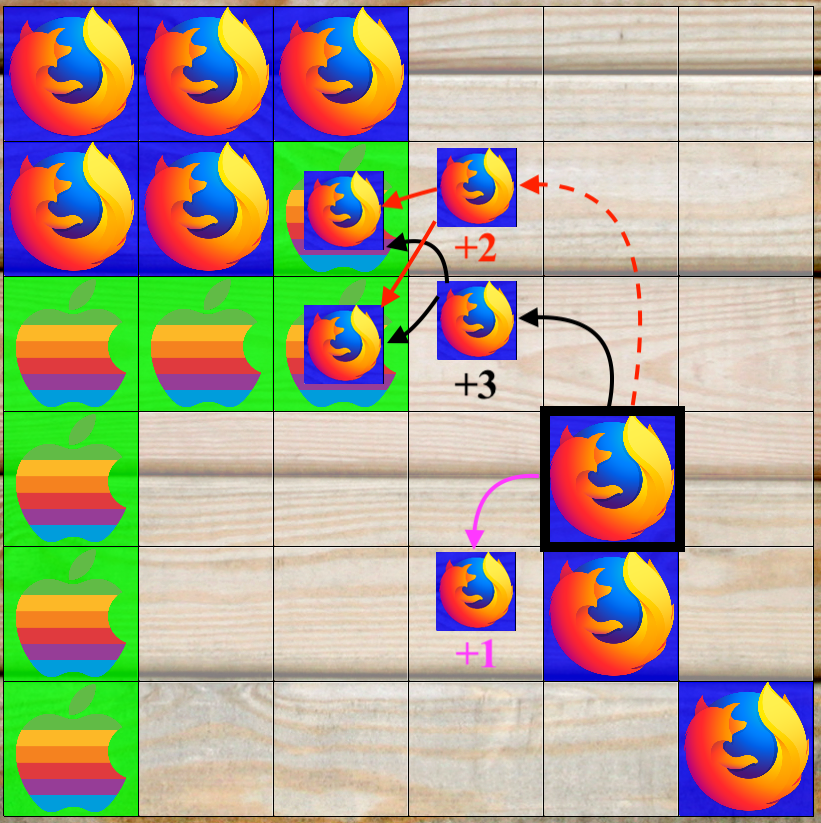
\includegraphics[width=0.9\textwidth]{figures/truc.png}
            \caption{3 coups possibles et valeurs associées}
        \end{center}
    \end{figure}
\end{column}

\end{columns}

\end{frame}

\subsection{Algorithme MinMax}

\begin{frame}[fragile]
\frametitle{\insertsectionhead : \insertsubsectionhead}
\begin{block}{MinMax}
Cet algorithme renvoie le meilleur coup que le joueur peut effectuer (en créant l’arbre des possibilités par récursion et le remontant en appliquant le max ou min si c’est le tour d’un ennemi ou d’un allié). 
\end{block}
\begin{figure}[h]
    \begin{center}
    \vspace{-5px}
    \caption{Exemple d’un arbre étiqueté avec les valeurs d'un MinMax (1/3) (Wikipédia)}
    \vspace{-5px}
    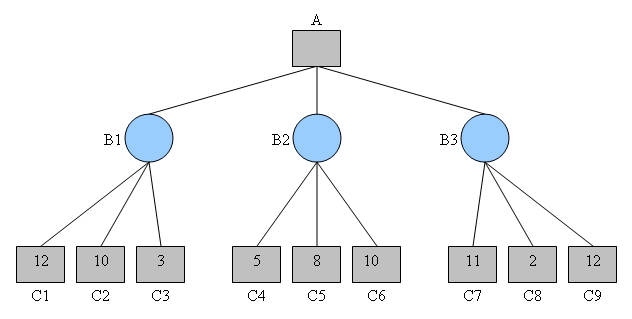
\includegraphics[width=0.8\textwidth]{figures/minmax1.png}
    \end{center}
\end{figure}
\end{frame}

\begin{frame}[fragile]
\frametitle{\insertsectionhead : \insertsubsectionhead}
\begin{block}{Valeurs des nœuds B}
Les nœuds B reçoivent chacun la valeur minimum stockée dans leurs fils C.
\end{block}
\begin{figure}[h]
    \begin{center}
    \vspace{-5px}
    \caption{Exemple d’un arbre étiqueté avec les valeurs d'un MinMax (2/3) (Wikipédia)}
    \vspace{-5px}
    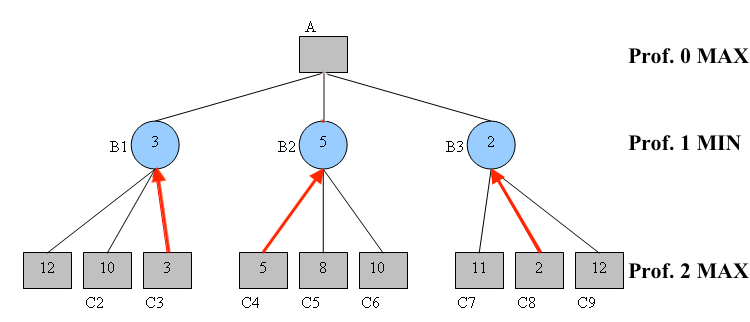
\includegraphics[width=1\textwidth]{figures/minmax2.png}
    \end{center}
\end{figure}
\end{frame}

\begin{frame}[fragile]
\frametitle{\insertsectionhead : \insertsubsectionhead}
\begin{block}{Valeur du nœud A}
Pour déterminer la valeur du nœud A, on choisit la valeur maximum de l’ensemble des nœuds B.
\end{block}
\begin{figure}[h]
    \begin{center}
    \vspace{-5px}
    \caption{Exemple d’un arbre étiqueté avec les valeurs d'un MinMax (3/3) (Wikipédia)}
    \vspace{-5px}
    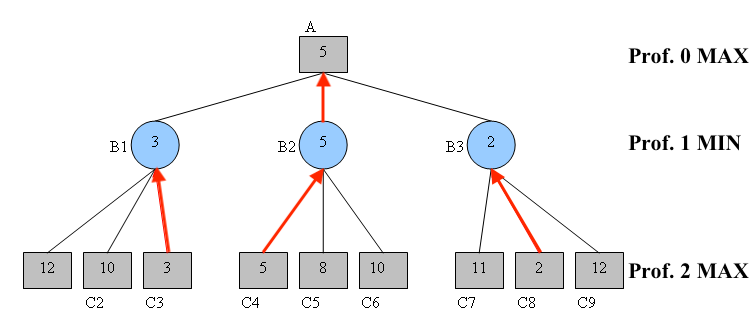
\includegraphics[width=1\textwidth]{figures/minmax3.png}
    \end{center}
\end{figure}
\end{frame}

\begin{frame}[fragile]
\frametitle{\insertsectionhead : \insertsubsectionhead}
\begin{figure}[h]
    \begin{center}
        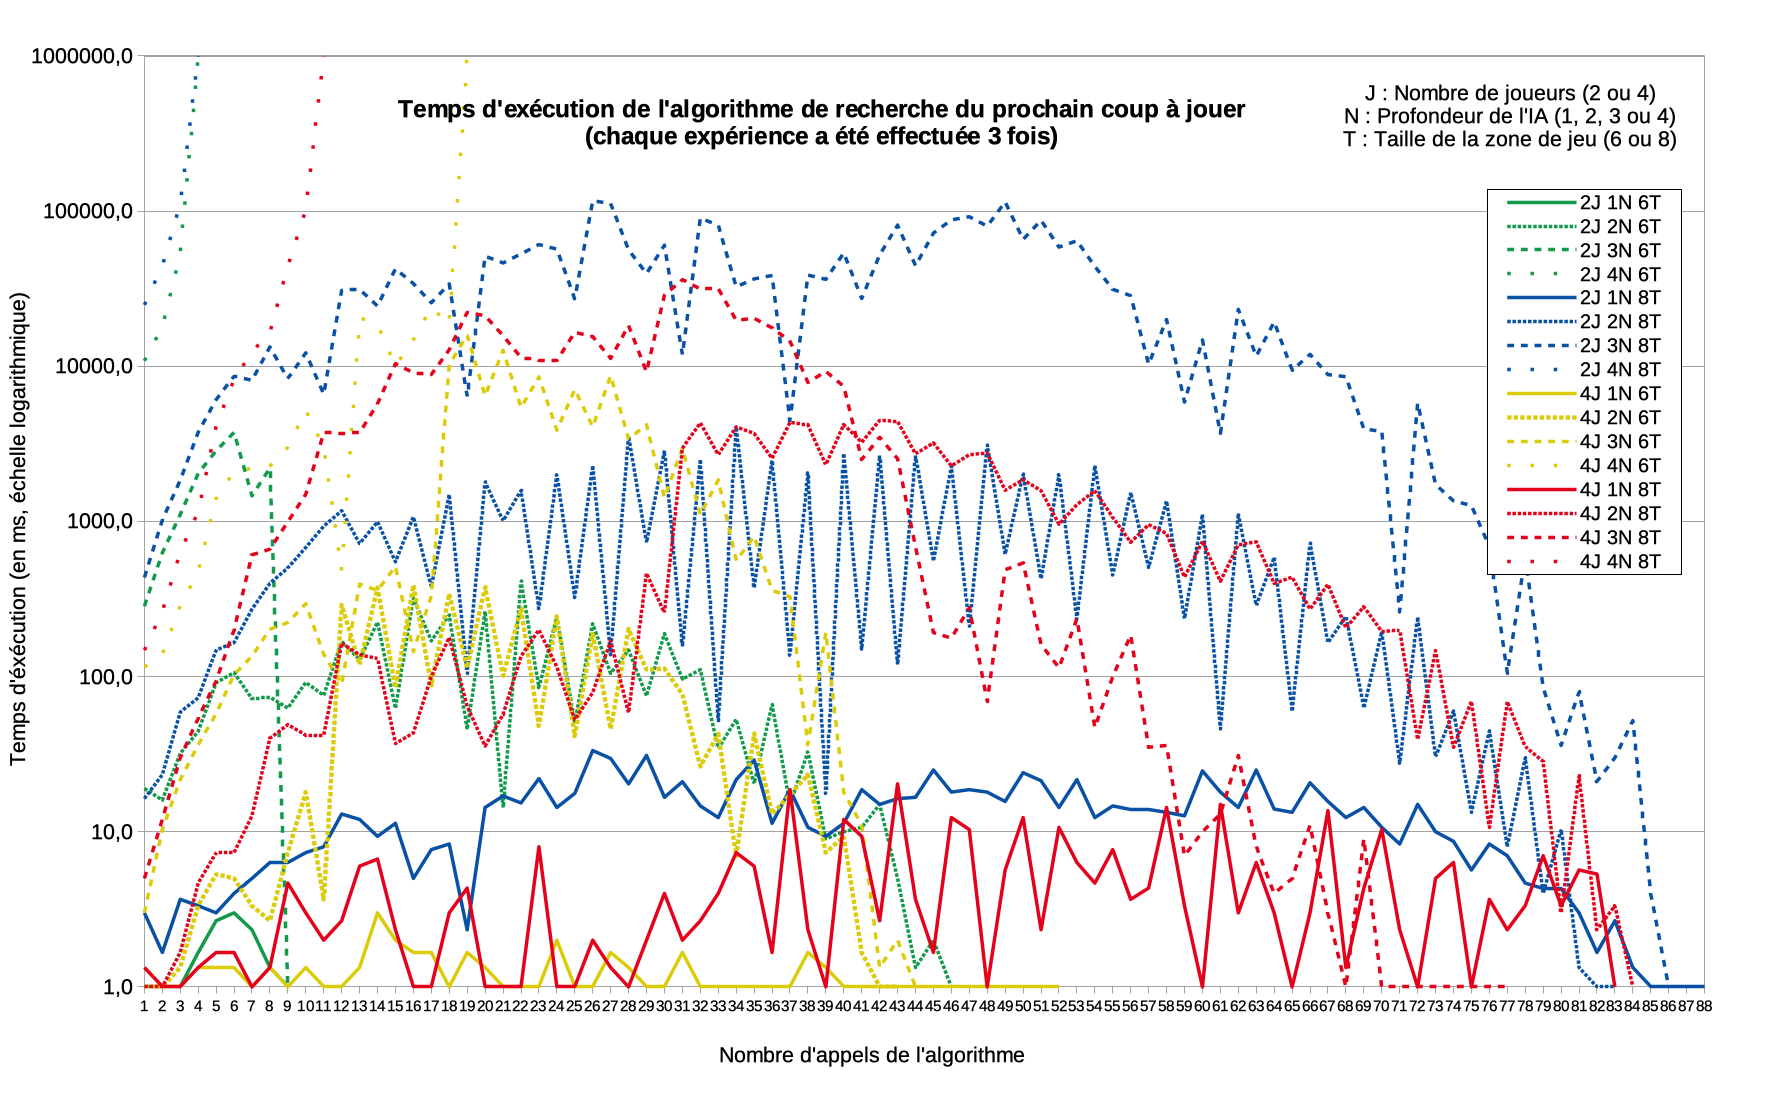
\includegraphics[width=1\textwidth]{figures/temps_exec.png}
        \vspace{-15px}
        \caption{Calculs de temps d'exécution de l’algorithme MinMax}
    \end{center}
\end{figure}
\end{frame}

\subsection{Élagage Alpha/Bêta de l'algorithme MinMax}

\begin{frame}[fragile]
\frametitle{\insertsectionhead : \insertsubsectionhead}
\begin{block}{Élagage Alpha/Bêta}
L’objectif de cette optimisation est de couper (ou élaguer) les branches de notre arbre pour avoir moins de contenu à explorer. Qui dit moins de contenu à explorer dit moins de calculs à effectuer. Cette opération est communément appelée un élagage.
\end{block}
\begin{figure}[h]
    \begin{center}
        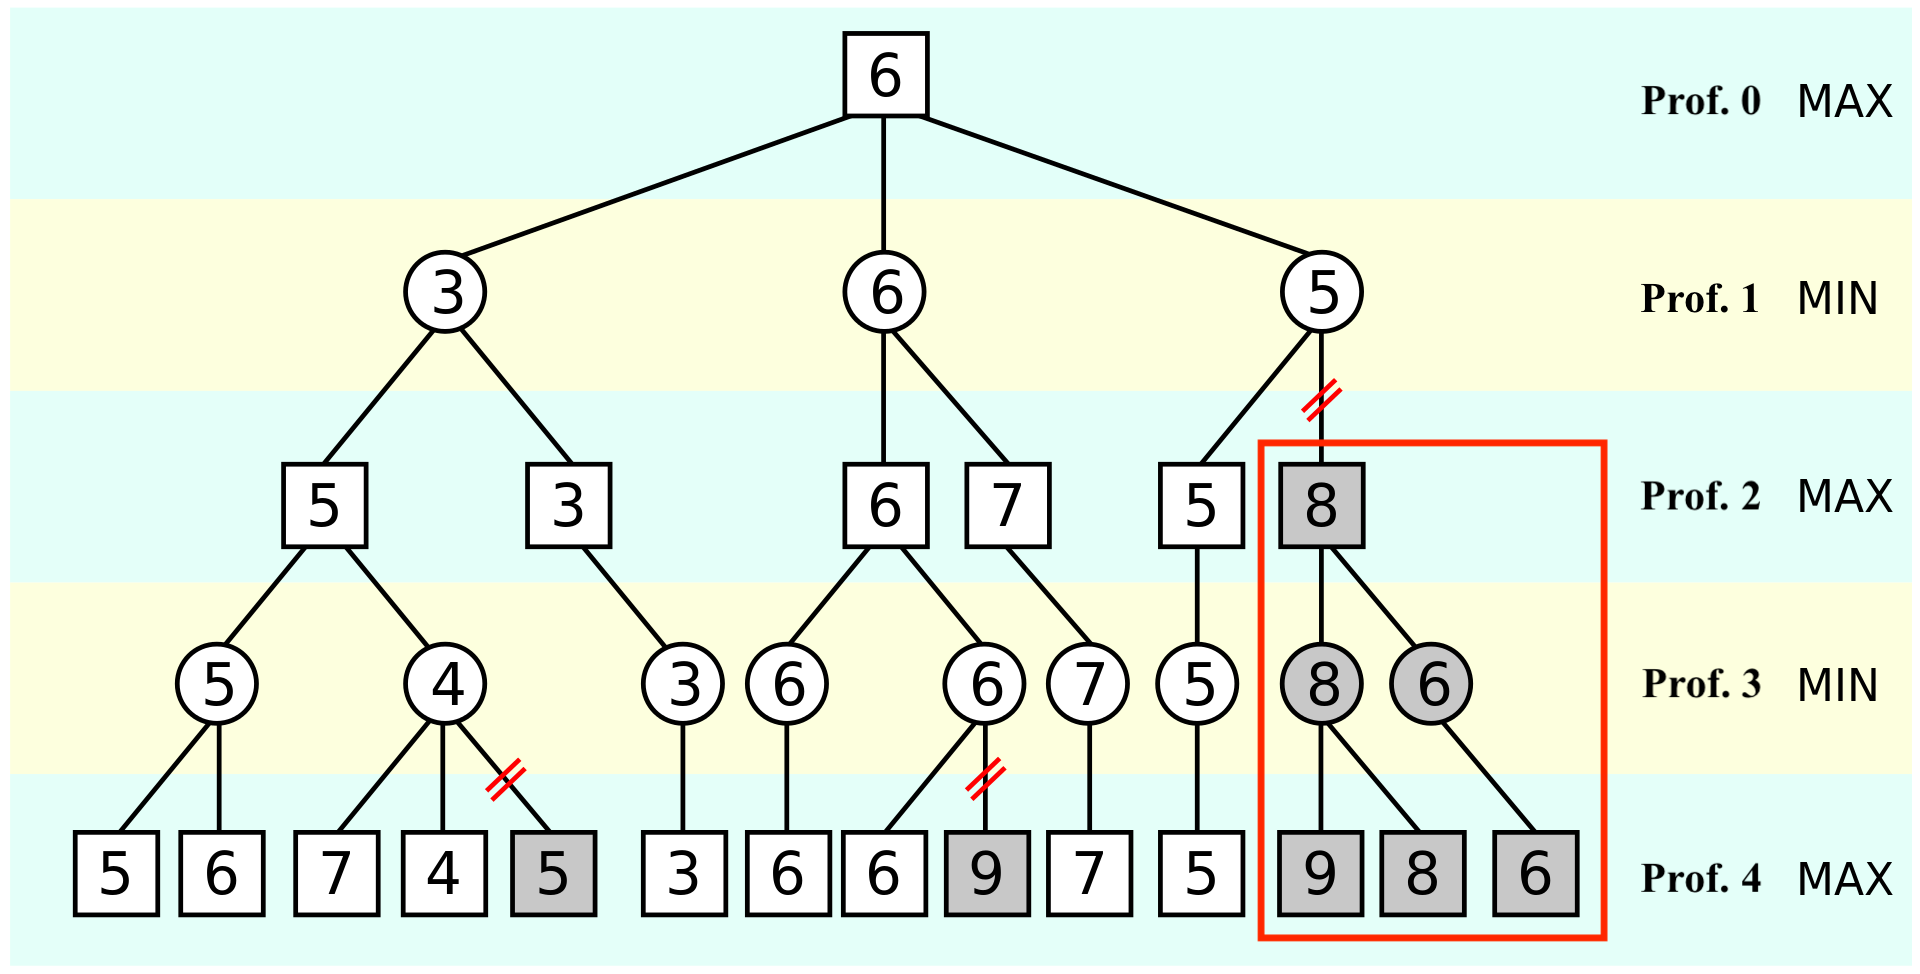
\includegraphics[width=0.8\textwidth]{figures/alphabeta.png}
        \vspace{-9px}
        \caption{Arbre étiqueté avec les valeurs d'un MinMax avec élagage Alpha/Bêta (Wikipédia)}
    \end{center}
\end{figure}
\end{frame}

\begin{frame}[fragile]
\frametitle{\insertsectionhead : \insertsubsectionhead}
\begin{figure}[h]
    \begin{center}
        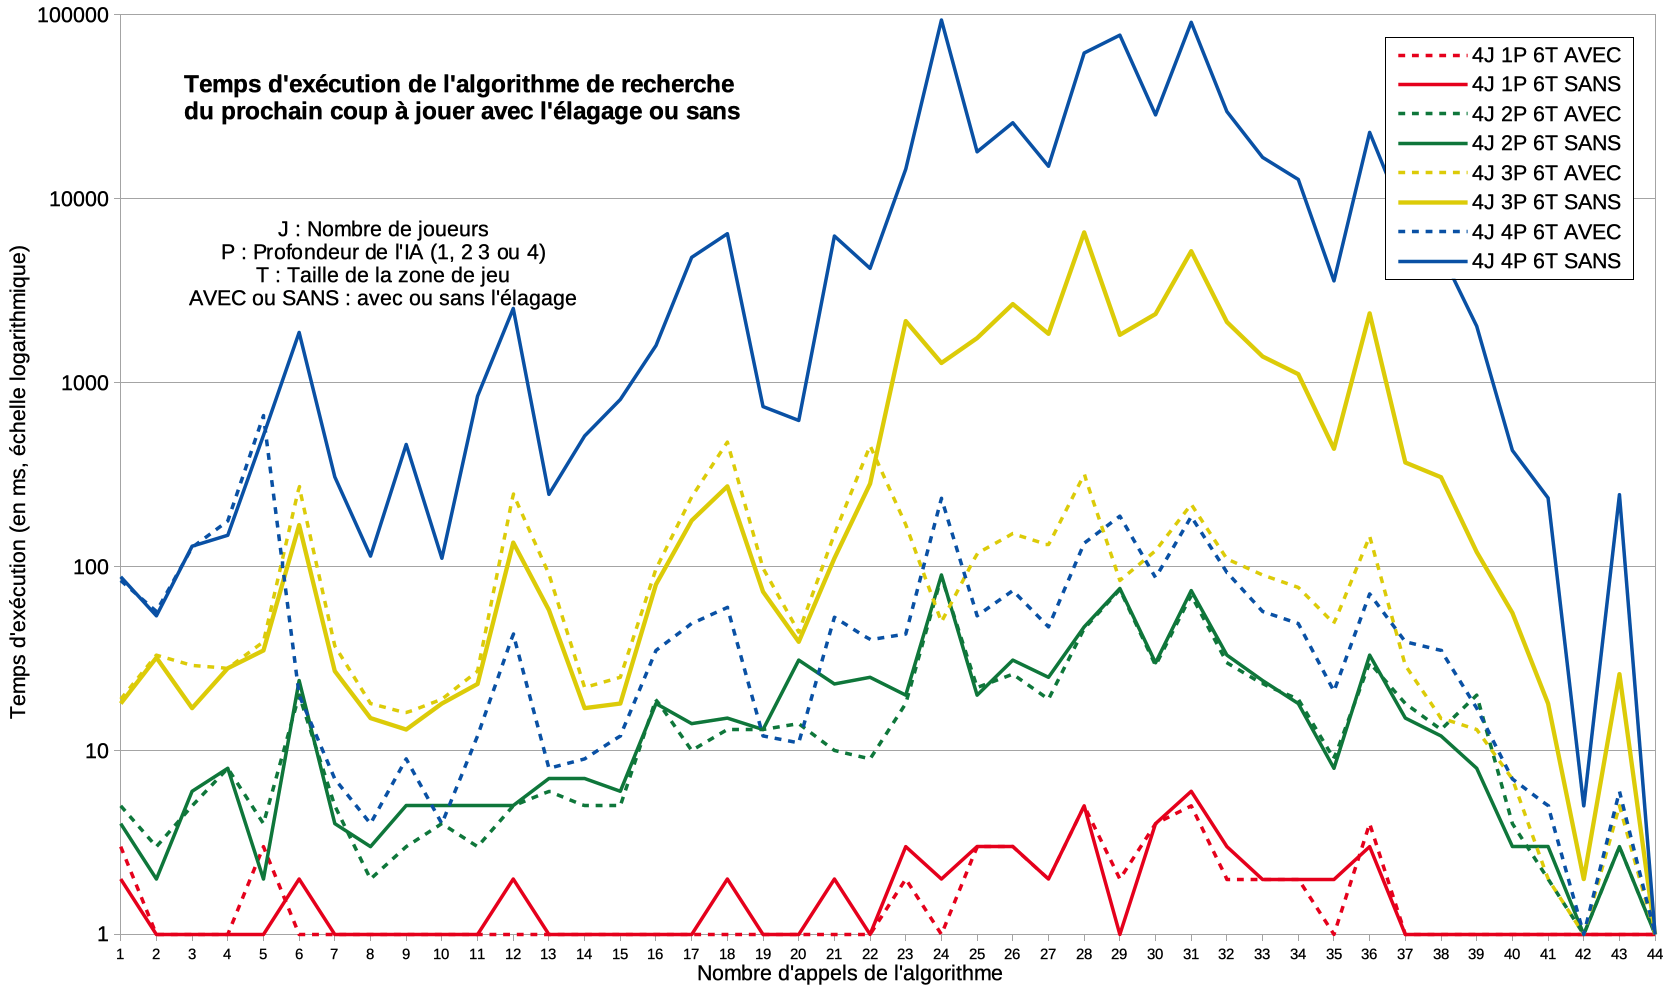
\includegraphics[width=1\textwidth]{figures/temps_exec2.png}
        \vspace{-8px}
        \caption{Calculs de temps d'exécution de l’algorithme MinMax avec ou sans élagage}
    \end{center}
\end{figure}
\end{frame}

\section{Conclusion}

\subsection{Compétences mises en œuvre et logiciels utilisés}

\begin{frame}[fragile]
\frametitle{\insertsectionhead : \insertsubsectionhead}

\includegraphics[width=1\textwidth]{figures/conclu.png}
\begin{itemize}
    \item Savoir s'organiser et se répartir le travail en groupe
    \item Utiliser des outils de travail adaptés (Librairie Slick2D, Gantt, Git, \LaTeX, Eclipse, ...)
    \item Mettre en pratique les connaissances des modules de L1 et L2
    \item Favoriser l'open-source et le gratuit
    \item Apprendre des autres et de leurs expériences
\end{itemize}
\end{frame}

\subsection{Diagramme de Gantt}

\begin{frame}[fragile]
\frametitle{\insertsectionhead : \insertsubsectionhead}
\begin{figure}[h]
    \begin{center}
        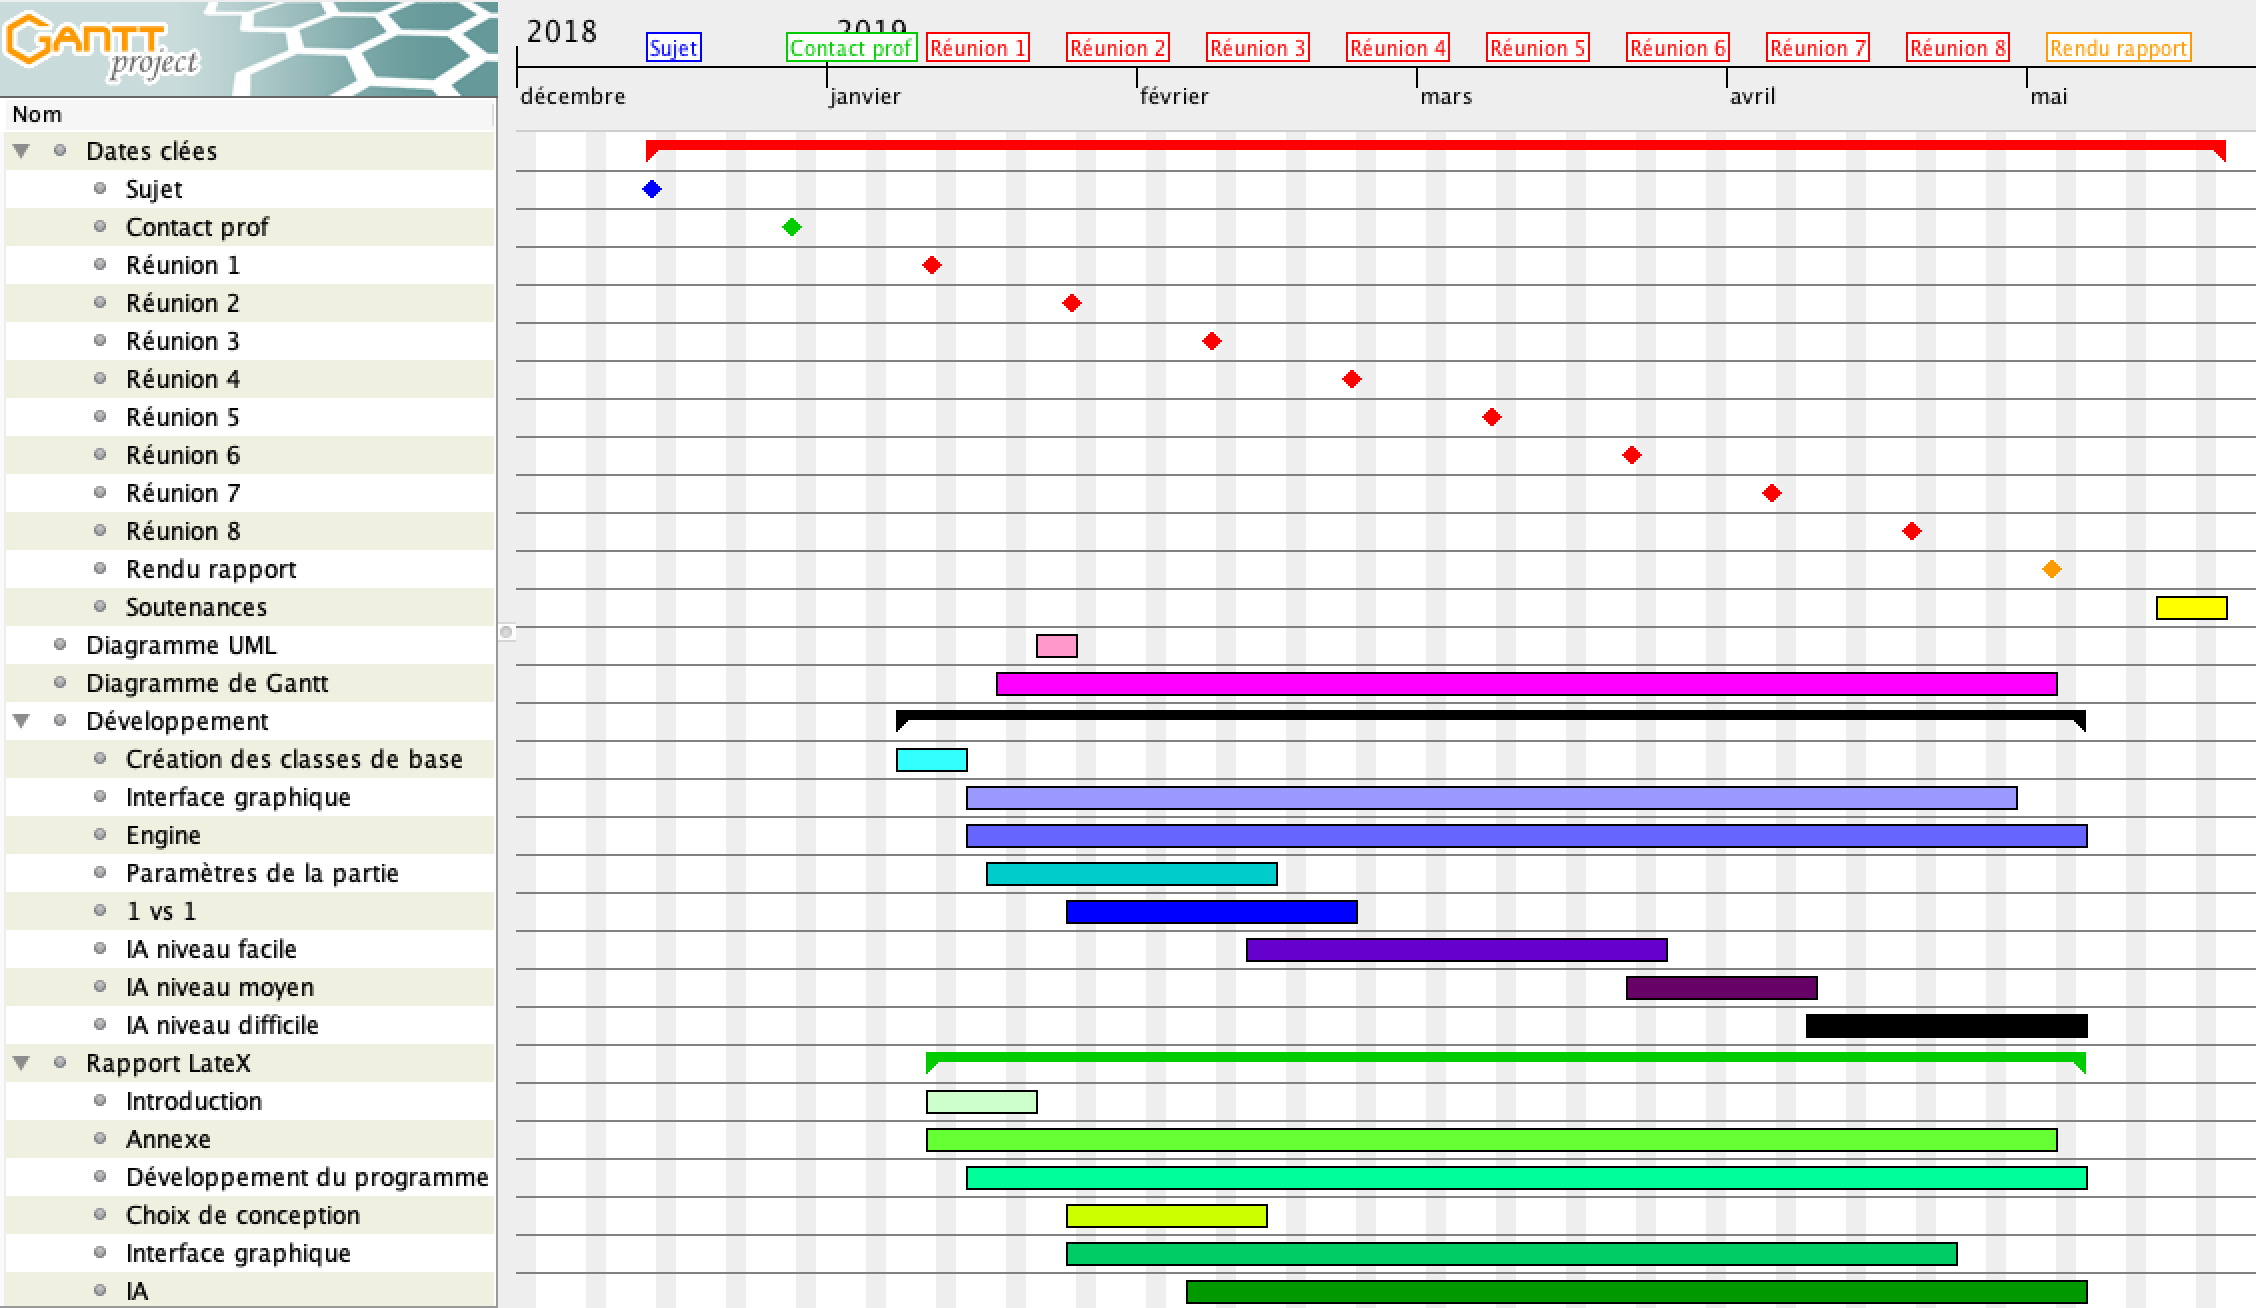
\includegraphics[width=1\textwidth]{figures/gantt.png}
        \vspace{-4px}
        \caption{Diagramme de Gantt de Blob Wars}
    \end{center}
\end{figure}
\end{frame}

\section{Ouverture}

\subsection{Comparaison de notre code avec l'exemple}

\begin{frame}[fragile]
\frametitle{\insertsectionhead : \insertsubsectionhead}
\begin{block}{Récupération du code du Blob Wars en ligne}
À l'aide du logiciel \textit{Sothink SWF Decompiler}, nous avons récupéré l'algorithme du jeu donné dans le sujet (Blob Wars en ligne). Il s'agit d'un enchaînement de boucles conditionnelles (\textit{If/Else}).
\end{block}
\begin{figure}[h]
\begin{center}
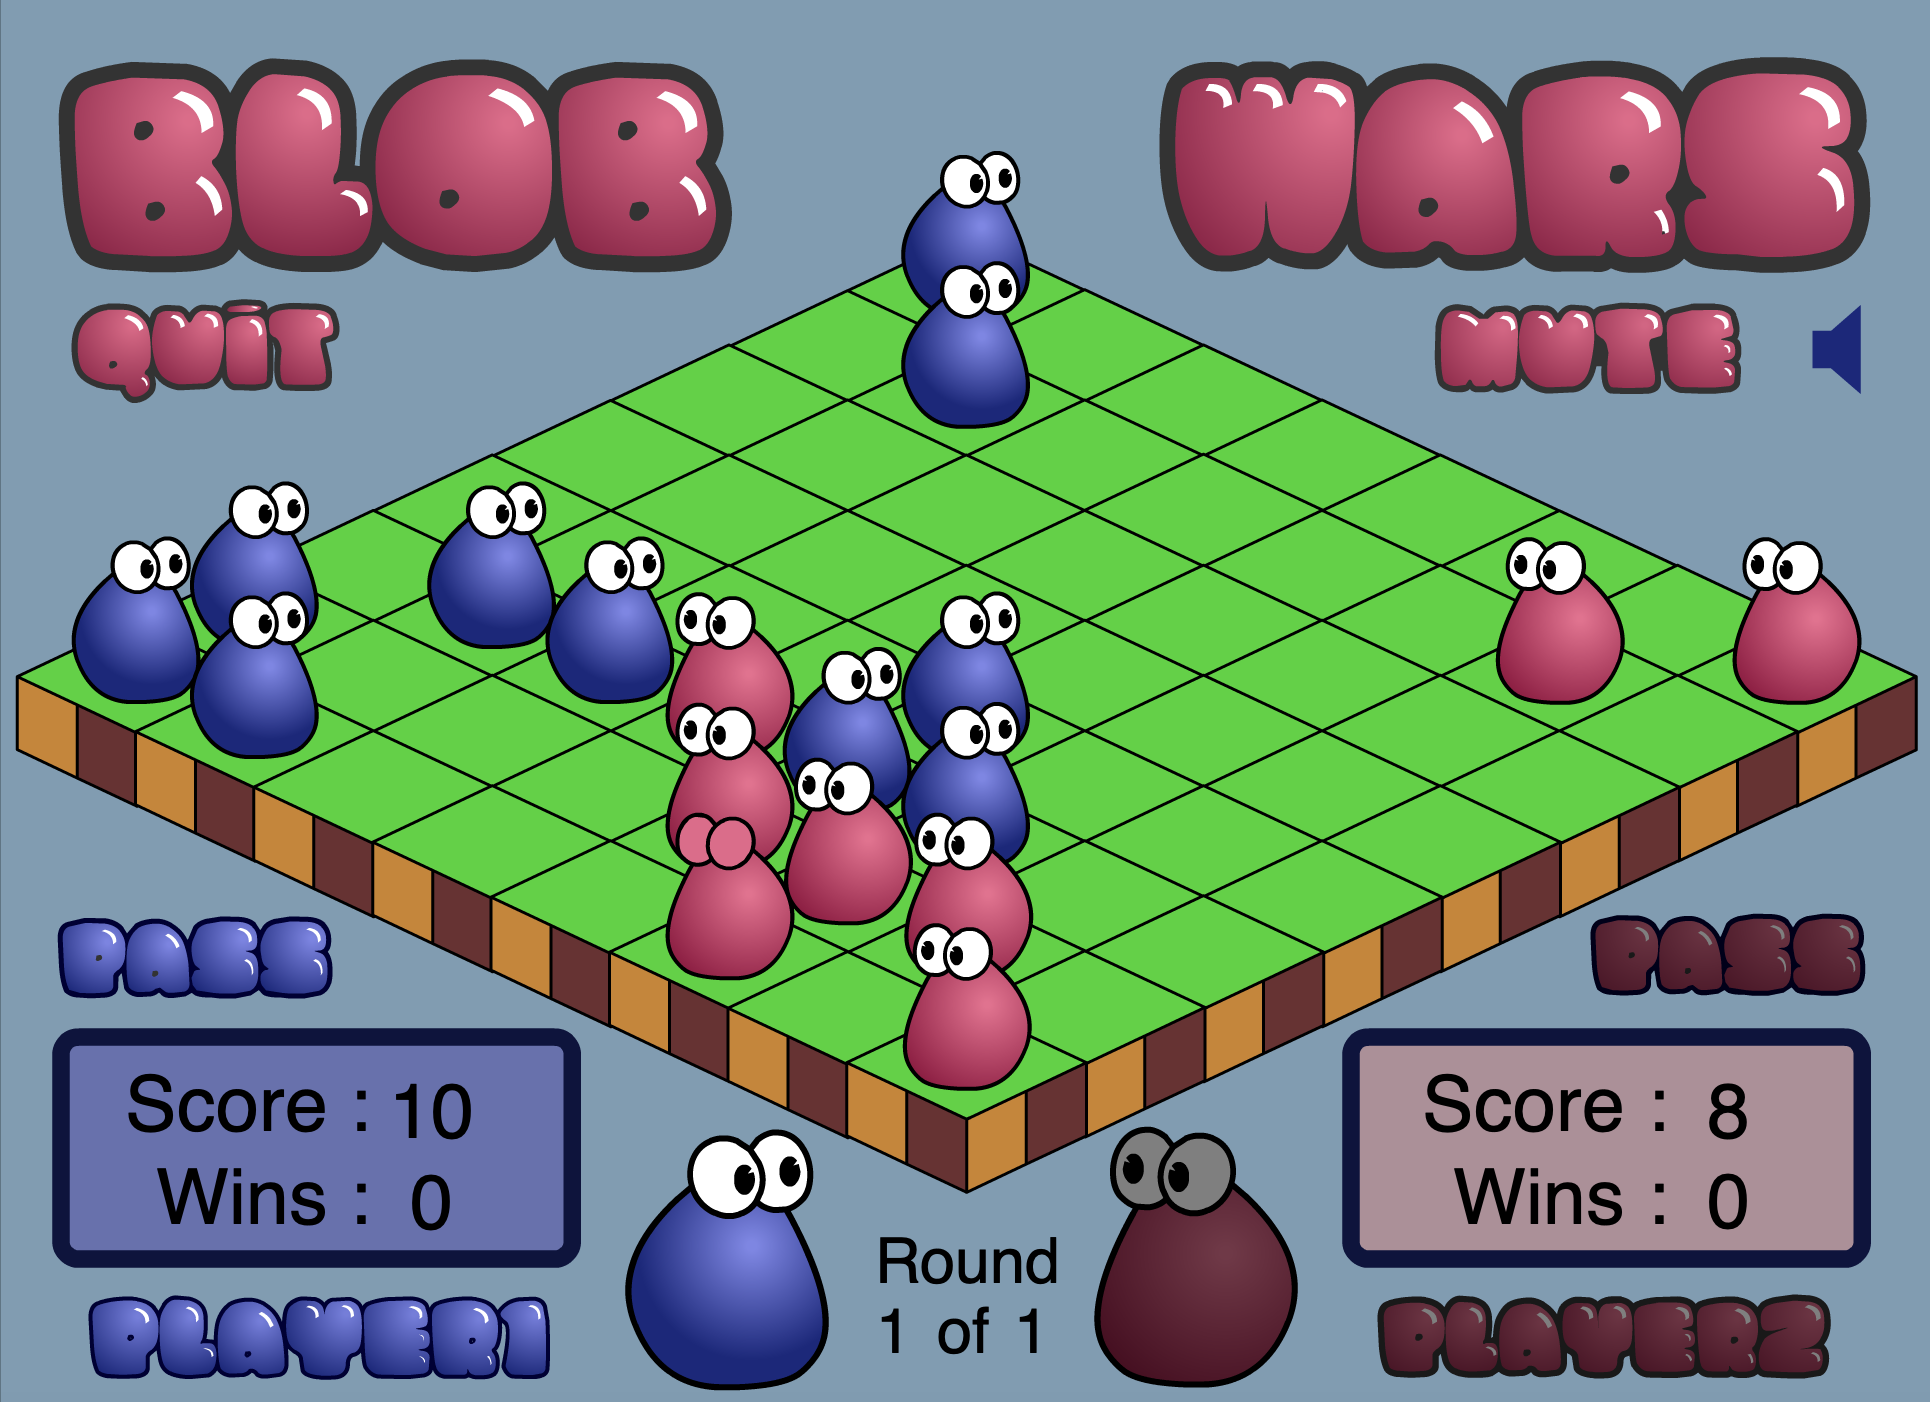
\includegraphics[width=0.5\textwidth]{captures/capture_ecran}
\caption{Capture d'écran du Blob Wars en ligne donné en exemple}
\end{center}
\end{figure}
\end{frame}

\subsection{Implémentations possibles}

\begin{frame}[fragile]
\frametitle{\insertsectionhead : \insertsubsectionhead}
\begin{itemize}
    \item Développement pour le web et/ou téléphone
    \vspace{3px}
    \item Pouvoir customiser l'apparence du jeu
    \vspace{3px}
    \item Ajouter des animations pour les pions
    \vspace{3px}
    \item Pouvoir sauvegarder pendant le calcul des nœuds
    \vspace{3px}
    \item Un bot qui pourrait jouer avec notre IA et contre l'IA du Blob Wars donné en exemple
    \vspace{3px}
    \item Ajouter d'autres fonctions d'évaluations
\end{itemize}
\end{frame}

\section{}

\begin{withoutheadline}

    % Premier transparent de titre
    \begin{frame}
      \titlepage
      \begin{minipage}[c]{.1\linewidth}
            \begin{center}
                
\includegraphics[width=2.5cm]{./figures/facSciences.png}
            \end{center}
       \end{minipage} 
       \hfill
       \begin{minipage}[c]{.46\linewidth}
            \begin{center}
                
\includegraphics[width=3cm]{./figures/icone.png}
            \end{center}
        \end{minipage}
        \begin{minipage}[c]{.26\linewidth}
            \begin{center}
                
\includegraphics[width=3.2cm]{./figures/umontpellier.png}
            \end{center}
        \end{minipage}
    \end{frame}
    
\end{withoutheadline}

\end{document}


%%%%%%%%%%%%%%%%%%%%%
A ne pas prendre en compte
%%%%%%%%%%%%%%%%%%%%%
Voir VERSUS
%%% Local Variables: 
%%% mode: latex
%%% TeX-master: "polycopieLatex"
%%% End: